% -*- latex -*-
%-----------------------------------------------------------------------
%;  Copyright (C) 2004
%;  Associated Universities, Inc. Washington DC, USA.
%;
%;  This program is free software; you can redistribute it and/or
%;  modify it under the terms of the GNU General Public License as
%;  published by the Free Software Foundation; either version 2 of
%;  the License, or (at your option) any later version.
%;
%;  This program is distributed in the hope that it will be useful,
%;  but WITHOUT ANY WARRANTY; without even the implied warranty of
%;  MERCHANTABILITY or FITNESS FOR A PARTICULAR PURPOSE.  See the
%;  GNU General Public License for more details.
%;
%;  You should have received a copy of the GNU General Public
%;  License along with this program; if not, write to the Free
%;  Software Foundation, Inc., 675 Massachusetts Ave, Cambridge,
%;  MA 02139, USA.
%;
%;  Correspondence concerning AIPS should be addressed as follows:
%;          Internet email: aipsmail@nrao.edu.
%;          Postal address: AIPS Project Office
%;                          National Radio Astronomy Observatory
%;                          520 Edgemont Road
%;                          Charlottesville, VA 22903-2475 USA
%-----------------------------------------------------------------------
%Body of intermediate AIPSletter for 31 December 2003

\documentclass[twoside]{article}
\usepackage{graphics}

\newcommand{\AIPRELEASE}{June 30, 2004}
\newcommand{\AIPVOLUME}{Volume XXIV}
\newcommand{\AIPNUMBER}{Number 1}
\newcommand{\RELEASENAME}{{\tt 31DEC04}}
\newcommand{\NEWNAME}{{\tt 31DEC04}}
\newcommand{\OLDNAME}{{\tt 31DEC03}}

%macros and title page format for the \AIPS\ letter.
\input LET98.MAC
%\input psfig

\newcommand{\MYSpace}{-11pt}

\normalstyle

\section{General developments in \AIPS}

\subsection{Compilers}

Instructions for fetching and installing the GNU 2.95.3 compiler are
given on the \AIPS\ web page.  The tar file is directly available from
NRAO\@.  This is needed since the 2.96.x compiler, shipped with some
versions of Linux, does not optimize code properly.  Users of more
recent Linux versions, \eg\ RedHat 9, will probably want to use the
GNU 3.2.{\it x} compiler which comes with it.  There have been reports
of failures with the GNU 3.3.3 and 3.3.4 compilers.  With the variety
of Linux flavors now appearing (although not yet at NRAO), we are less
certain about which works on what.

On Mac OS/X the IBM compiler has been found to produce executables
that run 50\%\ faster than those produced by current GNU compilers.
We are planning to buy --- they are far from free --- one of these
compilers and to make available a binary version for Macs.  This will
include regular updates via the MNJ, not just the frozen CD version.

\subsection{Current and future releases}

We now have formal \AIPS\ releases on an annual basis with binary
releases only for Solaris and Linux.  All architectures can do a full
installation from the source files.  The next release is called
\RELEASENAME\ and remains under active development.  You may fetch
(via \emph{anonymous} ftp over the Internet) and install a source-only
copy of this version at any time.  This \Aipsletter\ is intended to
advise you of developments to date in this new release.  Having
fetched \RELEASENAME, you may update your installation whenever you
want by running the so-called ``Midnight Job'' (MNJ) which uses
transaction files to copy and compile the code selectively based on
the code changes and compilations we have done.  There is a guide to
the install script and an \AIPS\ Manager FAQ page on the \AIPS\ web
site.

The MNJ has been changed.  It now serves up \AIPS\ incrementally using
the Unix tool {\tt cvs} running with anonymous ftp.  Linux sites will
almost certainly have {\tt cvs} installed; other sites may have
installed it along with other GNU tools.  Secondary MNJs will still be
possible using {\tt ssh} or {\tt rcp} or NFS as with previous
releases.  We have found that {\tt cvs} works very well, although it
has one quirk.  If a site modifies a file locally but in an
\AIPS-standard directory, {\tt cvs} will detect the modification and
attempt to reconcile the local version with the NRAO-supplied version.
This usually produces a file that will not compile or run as intended.

\AIPS\ is now copyright \copyright\ 1995 through 2004 by Associated
Universities, Inc., NRAO's parent corporation, but may be made freely
available under the terms of the Free Software Foundation's General
Public License (GPL)\@.  This means that User Agreements are no longer
required, that \AIPS\ may be obtained via anonymous ftp without
contacting NRAO, and that the software may be redistributed (and/or
modified), under certain conditions.  The full text of the GPL can be
found in the \texttt{15JUL95} \Aipsletter.

\section{Patch Distribution for \OLDNAME}

As before, important bug fixes and selected improvements in
\OLDNAME\ can be downloaded via the Web beginning at:

\begin{center}
\vskip -10pt
{\tt http://www.aoc.nrao.edu/aips/patch.html}
\vskip -10pt
\end{center}

Alternatively one can use {\it anonymous} \ftp\ to the NRAO server
{\tt ftp.aoc.nrao.edu}.  Documentation about patches to a release is
placed on this site at {\tt pub/software/aips/}{\it release-name} and
the code is placed in suitable subdirectories below this.  As bugs in
\NEWNAME\ are found, they are simply corrected since \NEWNAME\ remains
under development.  Corrections and additions are made with a midnight
job rather than with manual patches.  Remember, no matter when you
received your copy of \OLDNAME\ {\it you must} fetch and install its
patches if you require them.

The \OLDNAME\ release had a few important patches including a new one
in March.  These were:
\begin{enumerate}
\item\ {\tt DBCON} to handle more extension types for VLBI mostly
       {\it 2004-01-05}
\item\ {\tt FITLD} to handle FQ IDs correctly {\it 2004-01-08}
\item\ {\tt OHGEO} to handle transposed images correctly {\it
            2004-01-14}
\item\ {\tt CLIPM}, {\tt UVMLN} to get correct source numbers {\it
            2004-02-21}
\item\ {\tt EDITR} to correct the antenna numbers that end up flagged
            {\it 2004-03-03}
\end{enumerate}

\section{\AIPS\ Distribution}

We are now able to log apparent MNJ accesses and downloads of the tar
balls.  We count these by unique IP address.  Since dial-up
connections may be assigned different IP addresses at different times,
this will be a bit of an over-estimate of actual sites/computers.
We have abandoned the registration system since the software that
managed the database is broken and appeals to have it fixed have
fallen on deaf ears.  In 2004, there have been a total of more than
470 IP addresses so far that have accessed the NRAO cvs master.  Each
of these has at least installed \RELEASENAME\ and 143 appear to have
run the MNJ on \RELEASENAME\ at least occasionally.  During 2004 more
than 140 IP addresses have downloaded the frozen form of \OLDNAME,
while more than 465 IP addresses have downloaded \RELEASENAME\@.  The
attached figure shows the cumulative number of cvs access sites and
tar-ball download sites known to us as a function of week --- so far
--- in 2004.

\centerline{\resizebox{4in}{!}{\includegraphics{FIG/PLOTIT4a.PS}}}
\vfill\eject

\section{Using DVDs with \AIPS}

As the cost of the media drops and DVD drives proliferate around the
world it is worth considering how to use them for data storage in
general and in \AIPS\ specifically.  Most internal read/write drives
are priced at under \$200 and offer 4.7 GB storage on each disk
(typically priced at \$1 for a write-once disk DVD+/-R or \$2 for a
write-many  disk DVD+/-RW).  The price/GB ratio is better even than
inexpensive disk drives, and there are some other advantages like the
ability to easily distribute data to collaborators.  For more
information on  DVD burners and formats consult the DVD FAQ at
{\tt http://www.dvddemystified.com/dvdfaq.html}
Note that Sony and others have come out with dual-layer burners
that have 9 GB capacity.  The dual-layer disks are rather pricey
(\$10) at the time of this article, but price should fall quickly.
The Blu-ray format provides 25 GB capacity on a single layer disk, but
this format is expensive and incompatible with other DVD players.

There are essentially two different ways to write your \AIPS\ data to
DVD\@.  We first describe how to make an ISO formatted backup of an
\AIPS\ data area that can be mounted as a read-only disk.   Next we
describe how to create a UDF formatted disk that can be mounted either
read-only or read-write and used like any other \AIPS\ disk.

\begin{enumerate}
\item\ ISO.  For maximum compatibility with other machines a DVD+/-R
    or DVD+/-RW disk can use the ISO format.  Writing of these disks
    is typically done in a single session.  For example:

\begin{verbatim}
  % dvd+rw-format /dev/dvd  ! not necessary for DVD+R or DVD-R disks
  % growisofs -Z /dev/dvd -R -J /some/aips/directory
  % mount /mnt/dvd
  % ls /mnt/dvd             ! to see that its all there
  % ummount /mnt/dvd
\end{verbatim}

  To fill an entire disk should not take longer than 30 minutes, and
  for DVD+R should be done in under 16 minutes (burning at 4X). Note
  that you cannot remove or add new files to your ISO disk --- you
  have to rewrite it completely.

\item\ UDF. *** WARNING: Write-support for the UDF file system is
  listed as ``Dangerous'' in Linux 2.4.xx kernels.  Even if you apply
  the latest patch to your kernel, you may find that your machine does
  not communicate properly with your DVD burner.  Hopefully this
  situation will improve in the coming months, but in the meantime do
  not expect this option to work perfectly (or at all) on your system.
  ***

  DVD+RW disks can be formatted with a udf file system that allows them
  to be treated like a regular hard drive.  Files can be copied over
  with {\tt cp} and erased with {\tt rm}.  The drive can also be set
  up as an \AIPS\ disk so that files can be {\tt MOVE}d to it.  For
  more about using DVDs in \AIPS\ see also \AIPS\ Memo 109.  To mount
  a blank DVD+RW and make use of it use the following commands:

\begin{verbatim}
  % dvd+rw-format /dev/dvd   ! format
  % mkudffs /dev/dvd         ! make file system
  % mount /mnt/dvd
  % cp -r myfiles /mnt/dvd
    ...
  % umount /mnt/dvd
\end{verbatim}

  These disks can be read in read-only DVD drives so long as the UDF
  file system is available on the machine in question (generally true
  for all RedHat Linux machines).  Note that in some windows flavors
  this format is called DLA\@.  To fill an entire DVD+RW disk can take
  over an hour.  Also, note that UDF formatted DVD+RWs can only be
  mounted about 1000 times before they become permanently read-only
  (we guess --- we haven't tried this yet).

  If you want to create an \AIPS\ DVD and directly copy your data on
  your local machine to a DVD then you can do the following:

\begin{verbatim}
  % dvd+rw-format /dev/dvd  ! as above
  % mkudffs /dev/dvd        ! as above
  % mount /mnt/dvd          ! as above
  % mkdir /mnt/dvd/DA01
  % mkdir /mnt/dvd/DA01/FITS
  % touch /mnt/dvd/DA01/SPACE
  % chmod 755 /mnt/dvd/DA01/SPACE  ! builds an AIPS area on your DVD+RW
\end{verbatim}

  You will also have to have your AIPS administrator add an entry to
  {\tt DADEVS}.LIST that points to where the DVD is mounted ({\tt
  /mnt/dvd} in the above example).  Now after starting up {\tt AIPS}
  you should see your DVD as an \AIPS\ disk with 4588842 free blocks.
  You can use {\tt MOVE} to copy data onto the DVD, or {\tt UVCOP} and
  {\tt SUBIM}, or use it like any other (somewhat slow) \AIPS\ disk.
  If you see repeated errors from \AIPS\ while attempting to write
  files, or messages about ``permission denied'' when you attempt to
  do an {\tt ls} on the DVD, then your kernel is not communicating
  properly with the DVD burner.
\end{enumerate}

\section{Recent \AIPS\ and related Memoranda}

The following new \AIPS\ Memorandum is available from the \AIPS\ home
page.

\begin{tabular}{lp{5.8in}}
109 &  Using DVDs with \AIPS  \\
   &   Greg Taylor \&\ Eric W. Greisen (NRAO)\\
   &   January 20, 2004\\
   &   DVDs can be read and written by \AIPS\ using a udf file system
       on a DVD+RW device.  Once written, they can be used inside {\tt
       31DEC04} \AIPS\ when mounted on read-only DVD devices.  This
       capability also allows users to limit access for other users to
       their data areas.
\end{tabular}

\section{Improvements of interest to users in \RELEASENAME}

We expect to continue publishing the  \Aipsletter\ approximately every
six months along with the annual releases.  There have been a
surprising number of changes in \RELEASENAME.  A package of \AIPS\
procedures, called {\tt VLBAARCH}, to convert VLBA data from
correlator format to cleaned-up, single frequency-ID FITS {\it
uv}-table files, was added.  A new task {\tt ATMCA} was written to
determine atmosphere models from 2-4 calibration sources, applying the
result to calibrate data in phase-referencing experiments.  The new
task {\tt RLDIF} replaces the use of {\tt LISTR} by returning properly
averaged right minus left phase differences for use in polarization
calibration.  A new task {\tt FLAGR} flags data based on a variety of
criteria; a preliminary version of this task with algorithms based on
the rms within an integration time has been made available for
testing.  Another new task {\tt DSORC} is used to renumber sources
in a multi-source data set.  A surprisingly powerful verb {\tt SYSTEM}
was created to allow users to communicate to the host operating system
from within {\tt AIPS}\@.  A new verb and procedure {\tt RANDOM} and
{\tt GRANDOM} return random numbers for use in perturbing calibration
sequences or what have you.  Calibrator source models have been added
to the \AIPS\ distribution with a new verb {\tt CALDIR} written to list
available models and new tasks {\tt CALRD} and {\tt CALWR} to read and
write them.

\RELEASENAME\ uses a new numbering scheme for magnetic tape logical
unit numbers that is incompatible with previous versions.  Thus all
tape tasks and the server {\tt TPMON} must be from the same release.
Other than this, \RELEASENAME\ is compatible in all major ways with
the with the {\tt 15OCT98} and later releases.  There are significant
incompatibilities with older versions.

\subsection{UV data calibration}

\subsubsection{CALIB and FRING}

{\tt CALIB}, {\tt FRING}, and {\tt KRING} have traditionally
determined their solutions using disjoint time intervals.  Thus, for
example, data from the first minute are used for the first solution,
data from the second minute are used for the second solution, etc.
They have now been revised to allow solutions in overlapping
intervals.  Thus, one may use data from the first minute for the first
solution, data from 30 to 90 seconds for the second, data from 60 to
120 seconds for the third, etc.  This may help resolve phase
ambiguities in the case of high delay rates and provide more reliable
solutions without sacrificing some information about changes with
time.  An error in {\tt FRING} affecting data sets when the number of
working antennas increased in the middle was corrected.

{\tt CALIB} was changed to use the V polarization value in the source
table when calibrating RR (I+V) and LL (I-V).  This is particularly
useful for linearly-polarized feeds from equatorial telescopes such as
the WSRT\@.  For such telescopes the XX polarization is (I-Q) and the
YY is (I+Q) and Q is rarely zero for the usual calibrators.  By
changing the $uv$-data header from linear polarizations (Stokes -5 to
-8) to circular (Stokes -1 to -4) and telling {\tt SETJY} that the V
flux is -Q, {\tt CALIB} will now work for the parallel hands of WSRT
data.  This is stop-gap solution to the fact that \AIPS\ does not
solve the full polarization problem, but it does help.  {\tt CALIB}
does detect the user error in which the V flux is given as the same as
the I flux; it uses a V of 0 in that case.

The {\tt DOFIT} option in {\tt CALIB} was an attempt to use data from
all baselines but solve only for selected antennas.  This cannot work
since the corrections to antennas not being solved have to be known
anyway or those baselines cannot be used.  The difference between {\tt
DOFIT} and {\tt ANTENNAS} is no longer clear.  {\tt CALIB} briefly
forbade baseline-based solutions, but will now get solutions even if
only two antennas are used.  Users of this mode had better understand
what they are doing.

\subsubsection{Calibrator models}

Claire Chandler has offered models of basic calibrators from her web
site for some time.  To make these easier for \AIPS\ users to use
in their calibrations we have included these models with the \AIPS\
distribution.  The models are postage-stamp images with attached Clean
Components files in FITS format and are stored in the {\tt \$AIPSTARS}
directory.  The new verb {\tt CALDIR} will tell you about all {\tt
*.MODEL} files in this area.  Then you may use the new task {\tt
CALRD} to read in the model.  Note that you must use {\tt SETJY} to
write the total flux of your calibrator sources at your observing
frequency into the source table.  Then tell {\tt CALIB} to use the
model Clean Components for your calibrator.  It will automatically
scale the model to match the total flux in the source table.

At present, \AIPS\ supplies only the models prepared by Claire
Chandler.  They are of four sources, {\tt 3C48}, {\tt 3C138}, {\tt
3C147}, and {\tt 3C286}, at 3 frequency bands, K, Q, and U\@.  These
models should be good for all VLA configurations, but users should be
careful to switch their data to J2000 coordinates with {\tt UVFIX}
if needed before using them.

\subsubsection{Astrometric-level calibration}

Standard calibration techniques measure the instrumental/atmospheric
complex gain at one time and direction toward a calibrator source and
then apply those numbers to another time and direction for the target
source.  Interpolations in time may help deal with time variation, but
systematic effects due to the difference in elevation and azimuth of
the target and calibration sources remain.  The relatively new task
{\tt DELZN} was written to solve for residual elevation and clock
errors as a function of time.  It was given several new options: to
write an output text file at regular time intervals rather than those
in a {\tt CL} table, to write an output file with rate as well offset
information, to use phase delay rather than multi-band delay, and to
omit the clock solutions.

{\tt DELZN} requires closely-spaced observations of a number of
calibrators over a wide range in azimuth and elevation.  These
observations need to be repeated every few hours in order to provide a
measure of the change in the atmosphere and clocks over the observing
session.  A new task {\tt ATMCA} has been written to use observations
of two or more calibrator sources in the vicinity of the target source
to solve for the atmospheric delay as a function of coordinate and
time.  These solutions may then be applied at the coordinate and time
of the target source.  The {\tt CL} table is updated by {\tt ATMCA}
and a residual {\tt SN} table may be written.  This new method
requires that a lot of time be spent observing calibrators, but the
atmosphere often limits the accuracy of the observations otherwise.

\subsubsection{Other matters}

\begin{description}
\myitem{Model} division to determine gains was revised to change the
           weights correctly; previously the weights were multiplied
           by the model amplitude when the square of the model
           amplitude should have been used.
\myitem{CLCOR} was corrected for a sign error in the clock correction
           which changed phases and delays oppositely.  An {\tt ANTC}
           {\tt OPCODE} was added to do {\tt ANTP} but shifting the
           coordinates of epoch rather than the apparent coordinates.
           A {\tt TROP} {\tt OPCODE} was added to allow corrections
           from a file giving the total atmospheric zenith delay.  The
           {\tt ATMO} operation was fixed to use all the input data
           when the user is correcting both atmosphere and clock
           problems.
\myitem{CLCAL} was changed to enable a {\tt 2PT} interpolation on {\tt
           SELF} mode looping over source and using only those data
           suitable to the current source.  Previously it used only
           nearest neighbor values, a method now called {\tt SELN}\@.
           Errors due to missing data which affected the previous loop
           over sub-array as well as the new loop over source were
           found and corrected.
\myitem{RLDIF} is a new task to display the RL and conjugate LR phases
           on a printer, find the averages of the matrices, and return
           the phase correction in adverb {\tt CLCORPRM}\@.  In
           polarization calibration, it replaces the use of {\tt
           LISTR} which required the user to average different
           calibrator scans by eye and to type the printed result into
           the {\tt CLCOR} adverb.
\myitem{ELINT} was corrected to pass the {\tt CL} table phases through
           unchanged while correcting the amplitude.  Previously it
           zeroed the phases.
\myitem{SETJY} was changed to allow a user to change the Q, U, and V
           fluxes while leaving the I flux set by the {\tt CALC}
           function unchanged.
\myitem{SPLIT} and {\tt SPLAT} were fixed to find the correct
           frequency and $(u,v,w)$ scaling when averaging data across
           IFs as well as spectral channels.  The average frequency is
           is still not entirely accurate since it is a straight
           average while data averaging takes into account weights and
           flagging.  The {\tt AVIF} option was removed from {\tt
           AVSPC} since its ability to do multiple frequency IDs makes
           it prone to error.
\myitem{PCAL} was changed to find a reference antenna when {\tt
           REFANT} is not specified.  The attempt to avoid using a
           reference antenna was found to be unstable mathematically.
\myitem{VLACLCAL} \hspace{2em}  was corrected for the changes in the
           smoothing adverbs in {\tt CLCAL}\@.
\end{description}

\subsection{UV data handling}

\subsubsection{FILLM}

     The new archive system makes it very easy to download a very
mixed bag of data and users expect {\tt FILLM} to load it all in one
run.  To allow this a variety of changes were required.  The task now
reads any existing antenna table to make sure that the current
antennas match before concatenating the data.  It forces the I/O to do
a full re-open at each file boundary to insure that all needed data
streams are opened.  The test for using the Pie Town antenna at Q band
had an error that could lead to peculiar antenna files for Q-band
data.  {\tt FILLM} now allows the user to request {\tt CL} and {\tt
TY} intervals less than the apparent sample integration time.  This
can be important when data separated by 200 days or more are loaded;
times become less accurate and short scans may end up with no
corresponding {\tt CL} record.  A prejudice about using a source table
when no data had yet been accepted caused a source numbering error.
Errors reading short records at the ends of disk data files were also
corrected.

\subsubsection{Other matters}

\begin{description}
\myitem{DBCON} was changed to concatenate basic VLBI tables where
           appropriate, the buffers were made large enough to handle
           all tables, and the selection of which tables are copied
           was clarified.
\myitem{DSORC} is a new task to renumber sources in a multi-source
           data set.
\myitem{FITLD} was fixed to determine the maximum number of frequency
           IDs correctly and to use it in several places where the
           number of rows was used previously.  Source coordinate
           precession was made consistent with {\tt CLCOR}\@.
\myitem{Weather} tables are rather new and need to be copied correctly
           including selections on time, antennas number, and
           sub-array.  This copying was added to {\tt SPLAT}, {\tt
           FLGIT}, {\tt UJOIN}, and {\tt UVCOP}\@.
\myitem{VLBA} procedures {\tt VLBAFIX} and {\tt VLBASUBS} were changed
           to allow there to be multiple sub-arrays where appropriate.
\myitem{VLBAARCH} \hspace{2em} is a new collection of procedures to
           read data in correlator distribution format, to apply a
           variety of standard corrections, and then to write them out
           in \AIPS' {\it uv} table FITS format.  The analysts will
           use {\tt VLBAARCH} to simplify the distribution of VLBA
           data for our users.
\end{description}

\subsection{UV data editing}

\begin{description}
\myitem{FLAGR} is a new task released so far only in a preliminary
           form.  The current version measures the rms of $uv$ data in
           each time interval and flags those data with excessive rms
           either on a baseline or an antenna basis.  Other algorithms
           are currently under development.
\myitem{UVMLN} was fixed to place correct source numbers in the flag
           table; row number in the source table was confused with
           source number.
\myitem{CLIPM} was changed to allow flagging for too-low weights and
           was also corrected for the source-number error.
\myitem{EDITR} was fixed to put correct antenna numbers in the flag
           table when using {\tt NEXT BASELINE} and {\tt ENTER OTHER
           ANT} functions.  The correct antenna numbers appeared on
           the screen but not in the {\tt FG} table.
\myitem{SNFLG} was corrected to handle apparently large phase
           differences correctly.  Phases near 180 degrees with small
           differences were sometimes taken to have large differences
           and hence flagged.
\myitem{UVFND} was improved to allow the user to select which channels
           are tested for bad data separately from the selection of
           which channels are displayed.
\end{description}

\subsection{Imaging}

\begin{description}
\myitem{IMAGR} was corrected to suppress an infinite loop in the
           selection of the next field to image.  The flag that is set
           when a field has no components was not tested everywhere.
\myitem{WTMOD} was revised to allow weights to be modified for a
           single sub-array within the data set.
\myitem{SETFC} was revised to return adverbs {\tt NFIELD}, {\tt
           CELLSIZE}, and {\tt IMSIZE}\@.  This will allow pipelines
           to determine optimum imaging parameters and even do
           multi-facet imaging.
\end{description}

\subsection{Data display}

\begin{description}
\myitem{Printing} tasks and verbs were all changed to allow {\tt DOCRT
            = -2} to suppress form-feed characters and {\tt DOCRT =
            -3} to suppress most pagination and labeling when the
            printing is going to a text file rather than the printer.
            These options should make it easier to use the output text
            files as input to other programs.
\myitem{LISTR} was corrected (a) to do the vector sum on the two
            halves of the {\tt MATX} listing separately, (b) to
            display a phase rms properly computed for the phase+rms
            {\tt MATX} rather than giving an amplitude rms, (c) to
            scale phase displays in powers of 10, and (d) to allow
            {\tt GAIN} listings to include all sub-arrays.
\myitem{ISPEC} was fixed to print correct frequencies and velocities
            when the axis direction is inverted.
\myitem{PCNTR} was changed to allow any of the four images to be used
            for contouring and/or grey scale; previously the first
            image was used for contouring and for the I polarization
            cutoff image.  Bugs related to plotting both color
            polarization vectors and grey scales were corrected.
\myitem{VPLOT} was corrected to do cross-hand to parallel-hand ratio
            plots correctly (\eg\ {\tt POLPLOT='RL/RR'}); bad
            addressing reduced these previously to zero.
\myitem{UVPLT} was changed to do self-scaling on binned values where
            appropriate; previously it used un-binned data to set the
            scales even when only binned data were plotted.
\myitem{SNPLT} was revised to do a fixed $x$ scale plot when {\tt
            TIMERANG} is specified and was corrected to allow plotting
            of all sub-arrays.  {\tt WETHR} was also changed to do the
            fixed $x$ scale plot.
\myitem{POSSM} received its usual large share of corrections.  It was
            found to use a ``tape'' LUN which precipitated the
            overhaul of tape LUNs reported elsewhere.  The divide by
            channel zero option limited the users' adverbs for no
            reason and exhibited several failure modes.  An exactly
            constant amplitude or phase could cause nasty things to
            happen.  The labeling of velocities on reversed spectra
            in plots was wrong, although the text file output was
            okay.
\myitem{OFMFILE} standard files are displayed on a web site:
            {\tt http://www.nro.nao.ac.jp/$\sim$sawada/aipscb/}
\myitem{TVPSEUDO}\hspace{2em} was enhanced with yet another step function.
\end{description}

\subsection{Analysis}

\subsubsection{Gaussian fitting}

{\tt IMFIT} and {\tt JMFIT} received some attention over the last six
months.  They were revised to return the fit values in new adverbs
{\tt FMAX}, {\tt FPOS}, and {\tt FWIDTH} and to return the
uncertainties in the {\tt DOMAX}, {\tt DOPOS}, and  {\tt DOWIDTH}
adverbs.  The adverb {\tt RADIUS} was added to these tasks to define a
radius over which the true image rms should be found (rather than
using the full image).  It can also be used to force a particular
value for the image rms.  Errors affecting the deconvolved widths were
found, especially in the ``maximum'' and, more generally, in {\tt
IMFIT}\@.  The fitting for true rms was changed to ignore pixel values
that are pure 0.0, assuming that these are probably {\tt REMAG}ed
blanked pixels rather than true zeros.

{\tt SAD}'s printed output is sorted into user-chosen order.
Additional choices of order were added and all were made to use
correct values even in the presence of rotation.  The number of
allowed components was raised to 40000 and an option to expand or
shrink the fit window was added.  The default ({\tt DPARM(10) = 0})
was found, however, to be a good choice.  An option to use the
bandwidth smearing in fitting, but not in the display of peak flux,
was added.  A significant error in position angles of
bandwidth-smeared Gaussians was corrected.  This affected initial
guesses and, more importantly, deconvolved Gaussians.  Fixes to the
maximum values in the deconvolution were also made.  Pure-zero pixels
are now also ignored in fitting for the image rms.

\subsubsection{Miscellaneous}
\begin{description}
\myitem{MFPRT} was revised to print in a format suitable as input to
            {\tt STARS} if desired.  It was fixed to use proper
            scaling for the fluxes and sexagesimal format for
            coordinates.
\myitem{CONVL} was revised to allow blanked pixels in the input image.
            They are Fourier transformed as zeros and then,
            optionally, re-blanked.
\myitem{OHGEO} was corrected to handle different transpositions in the
            input and master images; previously it assumed that the
            $x$ coordinates of both were of the same type.
\myitem{XTRAN} was changed to allow comment lines in the input file
            and to handle errors in the input file gracefully.
\myitem{TBOUT} was corrected to handle tables with more than 50
            columns; the \AIPS-wide limit is 128.
\myitem{IMDIST} was corrected (a) to give correct position angles
            under a wider variety of circumstances.
\end{description}

\subsection{Verbs, documentation, XAS}

\subsection{The \COOKBOOK\ and {\tt XHELP}}

The \COOKBOOK\ received a lot of attention in the last six months.  A
small part of the attention was to bring it up to date.  Chapters 4
and A were updated for {\tt RLDIF}, {\tt CLCOR}, {\tt CALRD}, and
\AIPS-supplied models, while Chapter 9 was updated for {\tt DELZN},
multi-band delays, {\tt CLCOR}, and {\tt AVSPC}\@.  All {\tt ABOUT}
files and Chapter 13 were updated as were the {\tt APROPOS} and {\tt
Tab}-completion data files.

Most of the changes were internal changes that are invisible in the
PostScript version of the \COOKBOOK\@.  They were done to allow us to
make fully cross-referenced versions in html and pdf formats.  This we
have done, making both versions available from the \COOKBOOK\ web
page {\tt html://www.aoc.nrao.edu/aips/cook.html}.  The pdf form is
rather large to load over the Internet, so we ship it as {\tt
\$AIPSPUBL/COOKBOOK.PDF}\@.   We recommend that you bring up your
local copy of the file in your favorite pdf reader such as {\tt
acroread}.

One of the reasons to use a local tool to display {\tt COOKBOOK.PDF}
is that it (and the html form) provide cross-references to every
\AIPS\ symbol via the {\tt XHELP} facility.  {\tt XHELP} itself is an
\AIPS\ verb that has been present for some time, but which had broken
with our move to Socorro.  This verb will access any \AIPS\ help file
loading it into your browser with links to the help files of any
\AIPS\ symbol found in that help file.  Over the last six months, we
have gotten this facility to work again and have removed a variety of
limitations in its capabilities.  It now handles symbols up to 10
characters in length, any number of symbols in each line, and even
does minimum match for symbols of 4 characters and more.  \AIPS'
``old-fashioned'' use of all capitol letters for its symbols is the
magic bullet that allows all of this to work with very few false
cross-references.

\subsubsection{Miscellaneous}
\begin{description}
\myitem{SYSTEM} is a new verb that allows the user to send a command
          to the host operating system.  There are no limits on the
          contents of the command string other than its 72-character
          length.  Output may be directed using another 72-character
          string; thus {\tt SYSCOM > SYSOUT} is sent to the operating
          system when {\tt SYSOUT} is not blank.  {\tt AIPS} waits for
          the command to finish and even receives an error code back.
          This verb may be useful in procedures to do something that a
          following \AIPS\ task or verb will need such as deleting a
          file that is not supposed to be there.  Note that you can
          even run another {\tt AIPS} with this verb.
\myitem{RANDOM} is a new verb which returns a random value evenly
          distributed between 0 and 1.  {\tt GRANDOM} is a new
          procedure that uses {\tt RANDOM} to return a
          Gaussian-distributed number with mean 0 and rms 1.  \POPS\
          has never encountered a verb that needs no arguments and
          returns one on the stack; for now {\tt RANDOM} requires a
          dummy argument must be provided although its value is
          ignored.
\myitem{LASTEXIT} \hspace{1em} is a {\tt SAVE}/{\tt GET} file that is
          automatically written when the user exits and read as the
          default vocabulary the the same user starts {\tt AIPS}
          again.  For some reason, this file can be damaged,
          particularly when the computer quits abruptly (``crashes'').
          We do not understand how this happens since the abort
          handler does not attempt to write this file, but we have
          worked to provide some damage control.  Now, when {\tt AIPS}
          starts, it will use a default \POPS\ vocabulary whenever an
          I/O error is found reading this file and whenever one of a
          couple simple symbol tests fail after the read.
\myitem{TGINDEX} and {\tt SGINDEX} and {\tt VGINDEX} verbs now sort
          their displays under control of the {\tt DOALPHA} adverb.
          The choices are no sort, date from most recent, and
          alphabetical.
\myitem{XAS} now offers a new option in the {\tt Xdefaults} file.  The
          screen size is now controlled by {\tt AIPStv*xPixels} and
          {\tt AIPStv*yPixels} with the default being the actual
          screen size less certain amounts for the borders.
\end{description}

\vfill\eject
\section{Improvements of interest to managers and programmers
in \RELEASENAME}

\subsection{Tapes}

In the early days of \AIPS\ we reserved logical unit numbers (LUNs)
from 31 through 30+NTPDEV for magnetic tapes and assumed that NTPDEV
would stay small.  When we also allowed LUNs up to only 50 as well
this led to a tension since we did not create a special dynamic
assignment of LUNs.  On most modern systems, NTPDEV is still small,
frequently being only 2 for remote tapes.  But some sites put all the
tape drives on one host, making NTPDEV quite large and causing some
tasks to fail if they use, \eg\ LUN 40.

Modern \AIPS\ permits all 128 LUNs allowed by operating systems to be
used.  Since no \AIPS\ tasks use the highest numbers, we have changed
the reserved tape LUNs to be 128 through 129-NTPDEV instead.  This was
relatively straightforward except for one problem.  Tasks of earlier
versions cannot talk to {\tt TPMON}s of {\tt 31DEC04} and vice versa.
This occasionally causes trouble at the moment, but, in time, this
difficulty will disappear.  Now sites with large numbers of tape
devices may use them all (up to 35) for \AIPS\@.

\subsection{Midnight Job}

In the past, when the Midnight Job (MNJ) detected changes to certain
files it sent ``special'' e-mails to alert managers to take specified
actions.  These included running {\tt POPSGN} when the {\tt POPS}
vocabulary changed and rebuilding {\tt XAS} when its code changed.  It
should have, but did not, include changes to certain system scripts
which have to be copied from {\tt \$SYSUNIX} to {\tt \$AIPS\_ROOT}
with a modification to define {\tt \$AIPS\_ROOT}\@.  Realizing
(finally) that these are very mechanical operations which are onerous
and confusing to many Managers, we have written a script called {\tt
UPDUPDATE} which will do all these things for you.  The \AIPS\ Manager
will still have to make changes ``by hand'' only in the very unlikely
case of changes to printer scripts, the Fortran pre-processor, and
{\tt READLINE}\@.

This new script will appear automagically in all systems installed
after it was written.  However, the \AIPS\ Manager of a pre-installed
{\tt 31DEC04} system will have to do one last thing by hand.  That is
to make a symbolic link in {\tt \$TST/\$ARCH/UPDATE} to {\tt
\$UPDUNIX/UPDUPDATE}\@.

\subsection{Other matters}

\begin{description}
\myitem{Read-only file systems} \hspace{6em} are now supported by
          \AIPS\@.  This was developed for DVDs as \AIPS\ disks, but
          has the attribute that any file system that is read-only to
          the current user may be used in \AIPS\@.  Besides the
          prohibition against file creation, deletion, and writing,
          the only loss from an \AIPS\ perspective is that the
          last-use date is not updated.
\myitem{install.pl} was changed to find the current machine in {\tt
          HOSTS.LIST}; previously the search always failed.
\myitem{START\_AIPS} \hspace{2em} was changed to deal better with the
          formats used to convey machine IP addresses in secure shell
          variables.
\myitem{START\_TVSERVERS} \hspace{7em} was adjusted still further.  It
          seems that quite a few computers cannot talk to themselves
          via the Internet, particularly when they are not connected.
          The use of {\tt \$DISPLAY = {\it hostname}:0} solves lots of
          problems with secure shell, but exposes these self-ignorant
          computers.  Where possible now we use {\tt \$DISPLAY = :0.0}
          which is fine except for those users that have more than one
          screen (and so want \eg\ {\tt :1.0}).
\myitem{CHARACTER} \hspace{2em} variables continue to confuse
          programmers in \AIPS\@.  Fortran compilers do odd things ---
          there are no rules in the standard --- with the character
          data and length variables.  For this reason, a Fortran {\tt
          CHARACTER} variable should never be passed to a subroutine
          which might be written in C\@.  This rule was ignored in
          quite a few Z routines, but has been fixed in case some new
          compiler does something different from the GNU standard.
          Another error that caused a task to fail is the declaring of
          lengths for {\tt CHARACTER} variables passed into a
          subroutine.  If the actual length passed is different, that
          length will be ignored and bad things can happen.
          Programmers should always use the length declaration {\tt
          *(*)} for passed {\tt CHARACTER} variables.
\end{description}
\vfill\eject

\section{\AIPS\ distribution statistics}

Since the registration system, always under-utilized, has now been
abandoned, we are left with analysis by IP address.  The table below
lists the IP addresses for 2004 by the final qualifier for shipments
of the {\tt 31DEC04} tarball, the {\tt 31DEC03} tarball, and access to
the cvs site.  The numbers in the cvs column include those sites that
install {\tt 31DEC04}, run a midnight job for {\tt 31DEC04}, or
run a final ``catch-up'' MNJ for {\tt 31DEC03}\@.

\vspace{10pt}
\begin{center}
\begin{tabular}{lrrrl}
\hline\hline
Code  & {\tt 31DEC04} & {\tt 31DEC03} & cvs site & Comments \\
\hline
 ar     &   - &  2 &   - & Argentina \\
 au     &  11 &  3 &  13 & Australia \\
 be     &   5 &  1 &   5 & Belgium \\
 br     &   2 &  1 &   3 & Brazil \\
 ca     &   9 &  1 &  12 & Canada \\
 cn     &   2 &  1 &   1 & China \\
 com    &  15 &  3 &   9 & USA commercial \\
 de     &   8 &  4 &   7 & Germany \\
 edu    & 105 & 25 & 119 & USA educational \\
 es     &  22 &  5 &  20 & Spain \\
 fi     &   5 &  - &   3 & Finland \\
 fr     &  11 &  3 &   7 & France \\
 gov    &  11 &  1 &   9 & USA government \\
 gr     &   1 &  - &   - & Greece \\
 hu     &   - &  - &   1 & Hungary \\
 ie     &   2 &  - &   - & Ireland \\
 in     &   4 &  2 &   2 & India \\
 it     &  19 &  7 &  17 & Italy \\
 jp     &  26 &  7 &  29 & Japan \\
 kr     &  10 &  2 &   9 & Korea (South) \\
 mil    &   6 &  2 &   4 & USA military \\
 mx     &   4 &  5 &   4 & Mexico \\
 net    &  30 &  9 &  22 & Network: usually service providers \\
 nl     &   8 &  1 &   7 & Netherlands \\
 nz     &   1 &  - &   1 & New Zealand \\
 org    &  10 &  1 &   8 & Non-commercial (non-profits) \\
 pl     &   5 &  2 &   5 & Poland \\
 pt     &   2 &  1 &   - & Portugal \\
 ru     &   4 &  2 &   3 & Russian Federation \\
 se     &   5 &  - &   4 & Sweden \\
 sk     &   1 &  - &   - & Slovak Republic \\
 tw     &   1 &  6 &   - & Taiwan \\
 ua     &   1 &  - &   - & Ukraine \\
 uk     &  19 & 10 &  15 & United Kingdom \\
 us     &   1 &  - &   - & USA \\
 za     &   - &  - &   2 & South Africa \\
 None   &  18 &  1 &  34 & No qualifiers, most NRAO not all \\
 Unknown&  82 & 33 &  96 & ``unknown host''  \\
 \hline
Total   & 466 &141 & 471 & \\
 \hline
\end{tabular}
\end{center}

%\section{Preview of coming attractions}
%\hphantom{.}
%\vfill
%\centerline{This page deliberately blank.}
\vfill\eject

% Order form and mailer page
% \cleardoublepage
\pagestyle{empty}
 \vbox to 4.4in{
  \vspace{12pt}
%  \vfill
  \centerline{\resizebox{!}{3.2in}{\includegraphics{FIG/Mandrill.eps}}}
%  \centerline{\rotatebox{-90}{\resizebox{!}{3.5in}{%
% \includegraphics{FIG/Mandrill.color.plt}}}}
  \vspace{12pt}
  \centerline{{\huge \tt \AIPRELEASE}}
  \vspace{12pt}
  \vfill}
\phantom{...}
\centerline{\resizebox{!}{!}{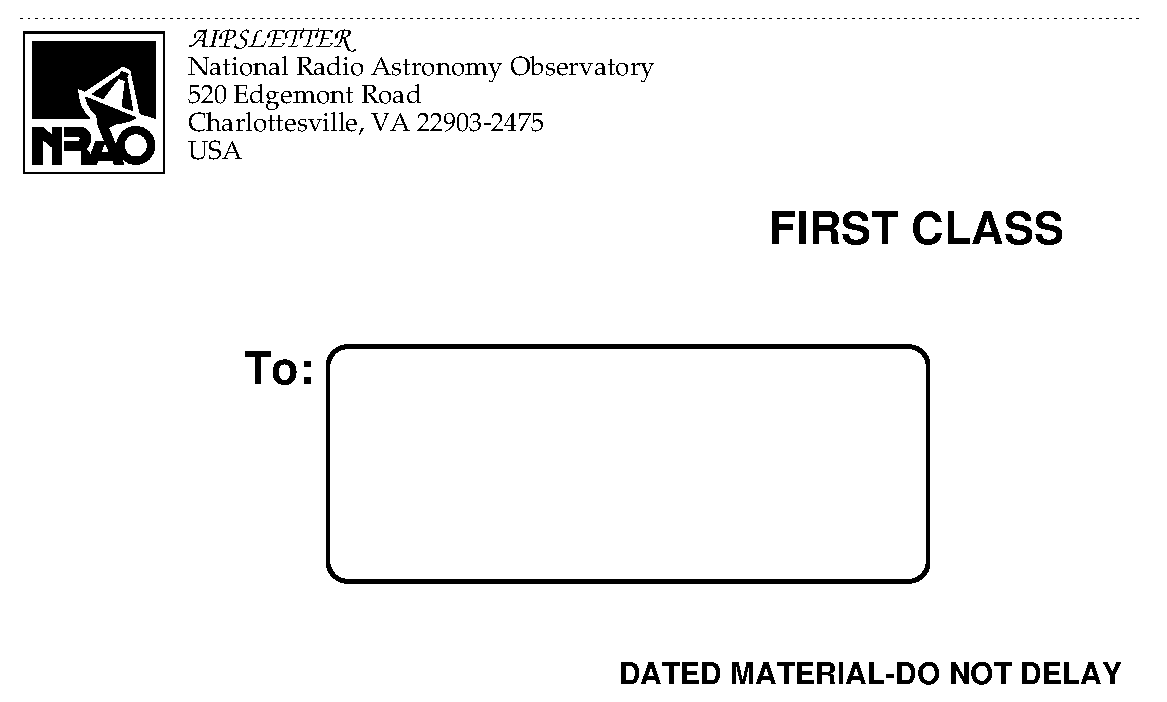
\includegraphics{FIG/AIPSLETM.PS}}}

\end{document}
